\subsection{Bombas}

\subsubsection{Altura Manométrica entre Dois Pontos}

A forma estendida da equação de Bernoulli é utilizada para avaliar as variações de carga (energia por unidade de peso do fluido) entre dois pontos de um duto de escoamento, incluindo perdas:

\begin{equation}
H = \frac{P_{2} - P_{1}}{\rho g} + \frac{V_{2}^{2} - V_{1}^{2}}{2 g} + z_{2} - z_{1} + h_f
\label{eq:bernoulli}
\end{equation}

Em que $H$ é a altura manométrica adicionada (se positiva) ou removida (se negativa) entre os pontos 1 e 2. Todos os termos da Equação \ref{eq:bernoulli} são expressos como carga hidráulica em metros: as pressões $P_1$ e $P_2$ usam unidades coerentes com $\rho$ e $g$ no termo $\frac{P_{2} - P_{1}}{\rho g}$; as velocidades $V_1$ e $V_2$ entram em $\mathrm{m/s}$; as cotas $z_1$ e $z_2$ são dadas em $\mathrm{m}$; e $h_f$ reúne as perdas distribuídas e localizadas em $\mathrm{m}$. Com essa convenção, perdas positivas aumentam a altura requerida pela bomba \cite{white2018}.

Essa equação é fundamental para avaliar a necessidade de bombeamento: uma bomba deve fornecer uma $H$ suficiente para superar as perdas e elevar o fluido da condição 1 até 2; inversamente, uma turbomáquina geradora extrairá essa energia do fluido.

\begin{figure}[H]
    \centering
    \caption{Cálculo da altura manométrica – Parte 1/2}
    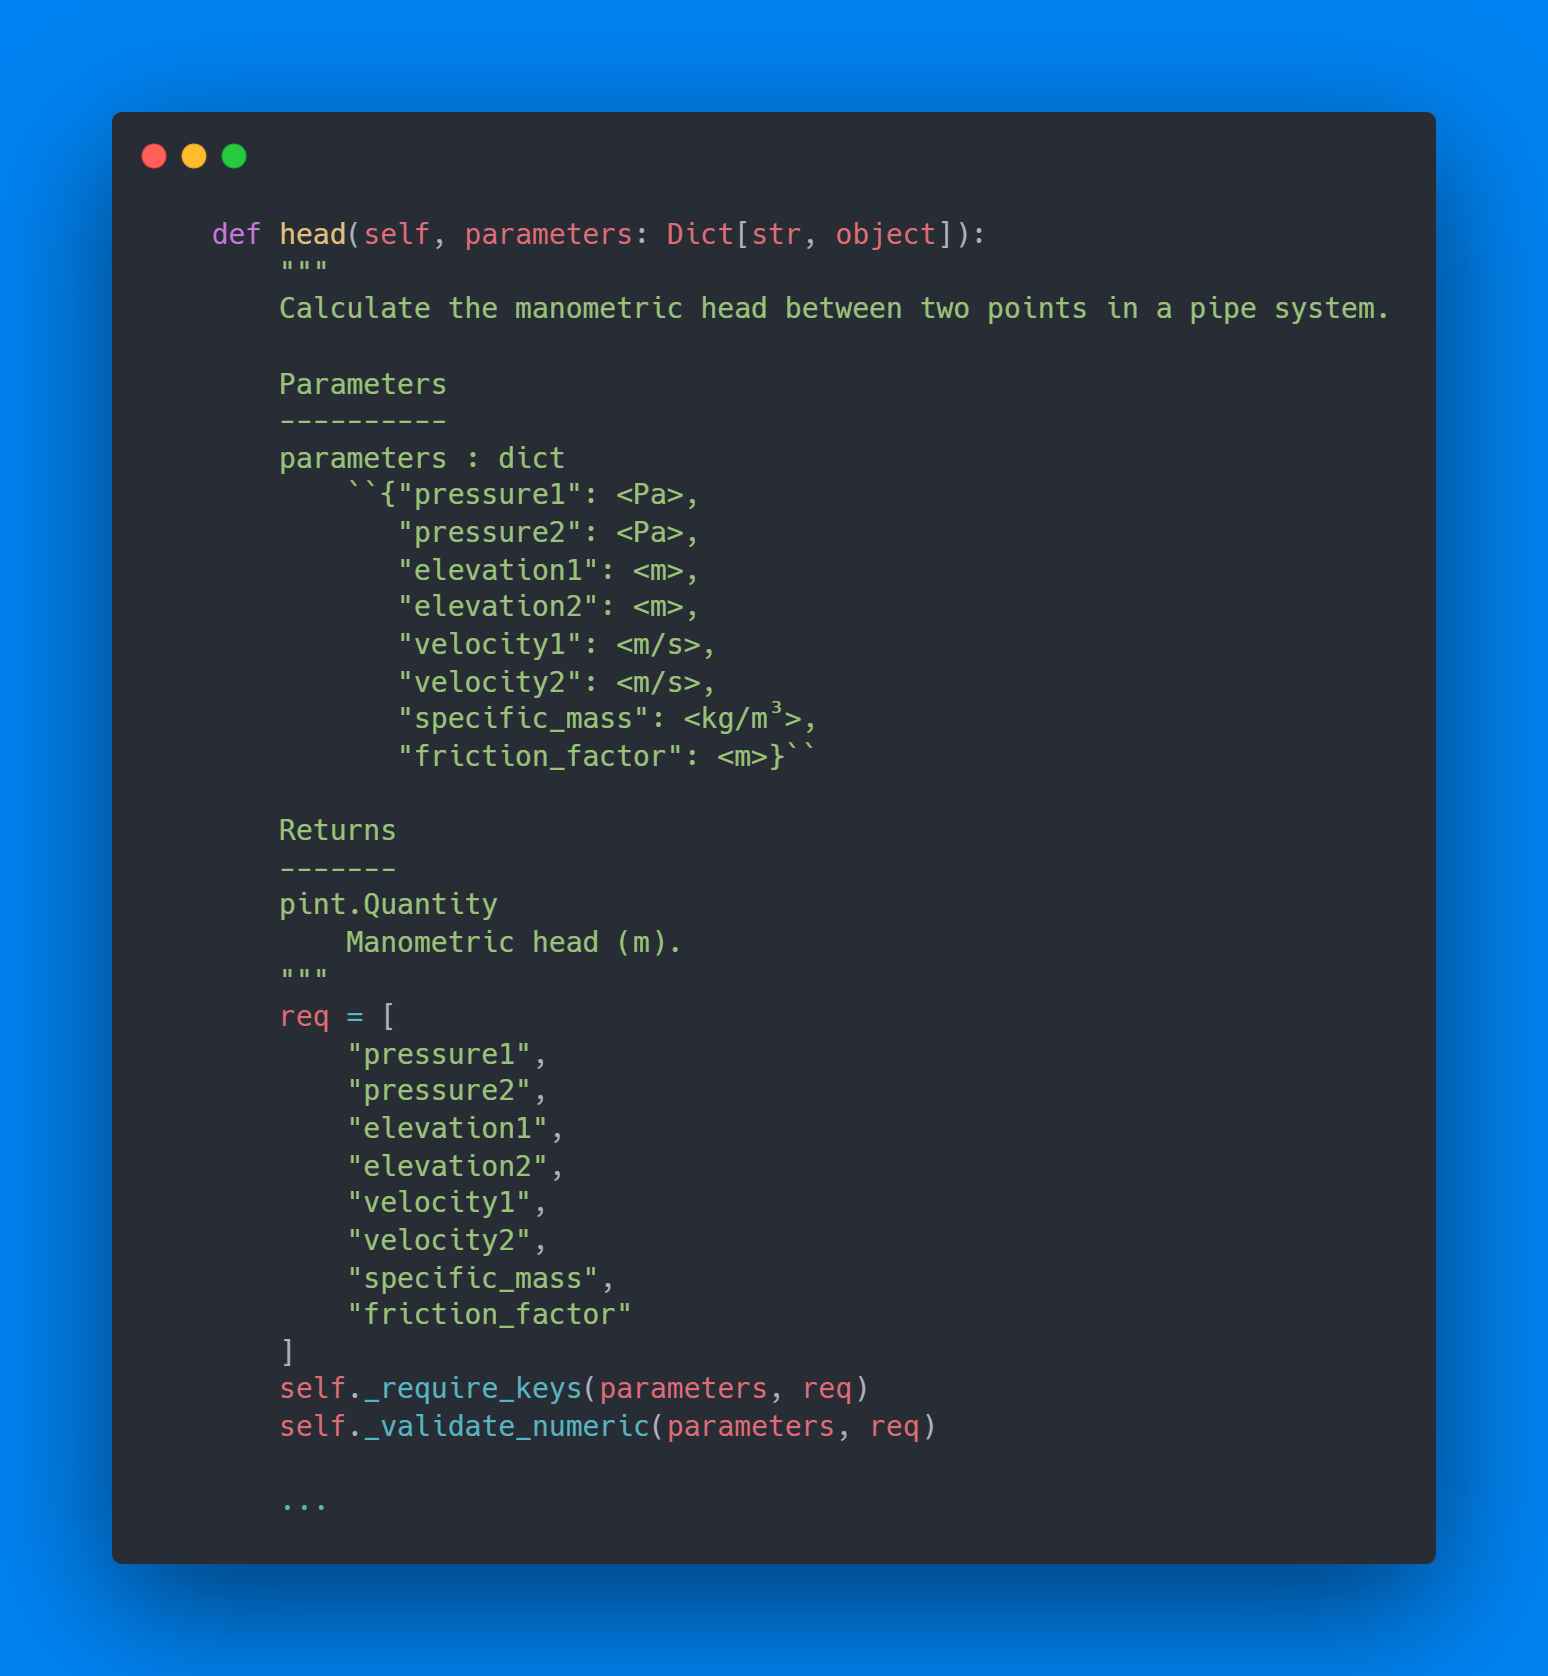
\includegraphics[width=\linewidth]{media/cap4_head_parte_um.png}
    \fonte{Elaboração própria (2026).}
\end{figure}
\begin{figure}[H]
    \centering
    \caption{Cálculo da altura manométrica – Parte 2/2}
    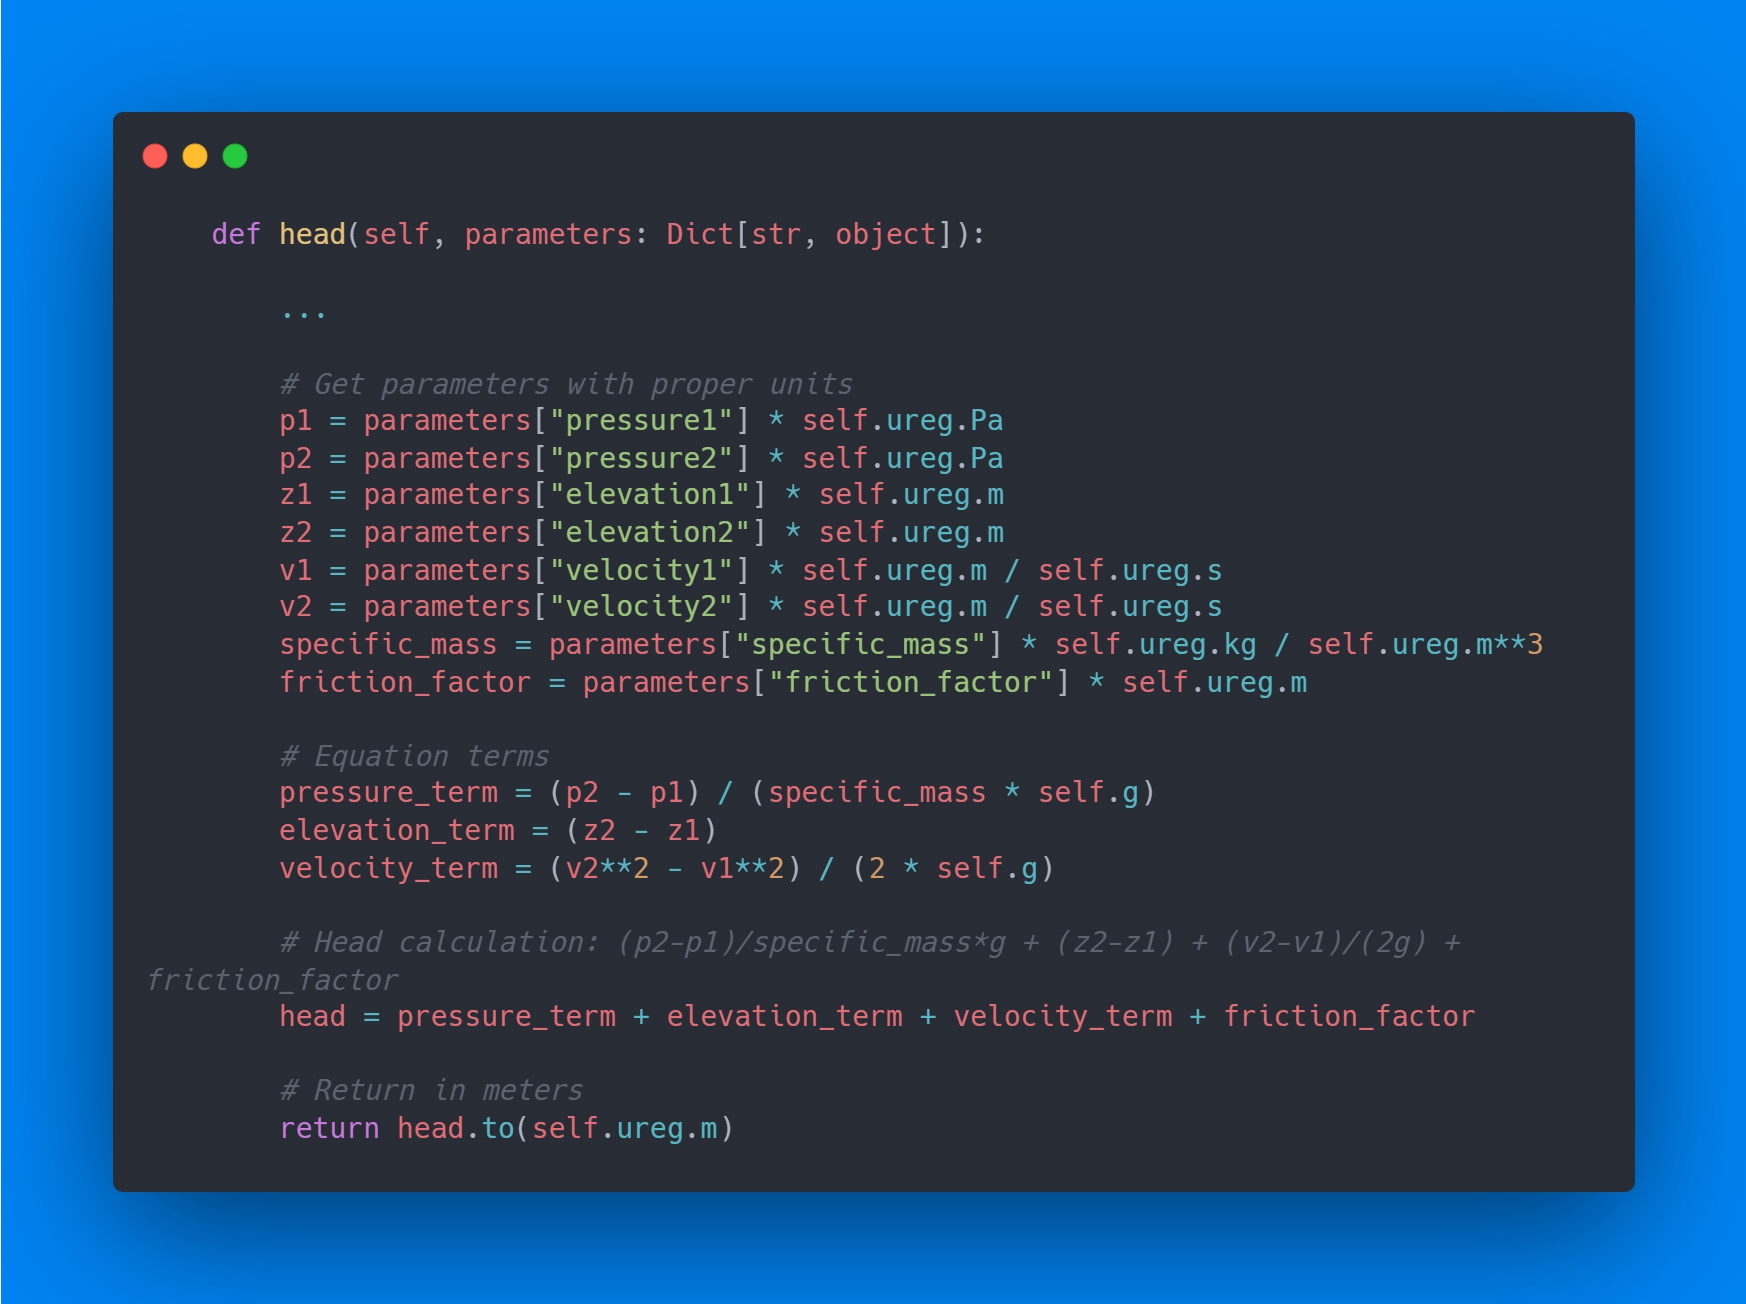
\includegraphics[width=\linewidth]{media/cap4_head_parte_dois.png}
    \fonte{Elaboração própria (2026).}
\end{figure}

\subsubsection{\textit{NPSH} Disponível}

Para evitar cavitação em bombas, calcula-se o \textit{NPSH} disponível na sucção, que deve exceder o \textit{NPSH} requerido pelo fabricante. A expressão para o \textit{NPSH} disponível, em termos de altura de líquido, é:

\begin{equation}
N P S H_{d i s p} = \frac{P_{s u c} + P_{a t m} - p_{v a p}}{\rho g} + \frac{V_{s u c}^{2} \ }{2 g} + \left( z_{s u c} - z_{0} \right) - h_{s u c}
\label{eq:npsh}
\end{equation}

O resultado da Equação \ref{eq:npsh} é expresso em metros de coluna do líquido bombeado. As pressões $P_{suc}$, $P_{atm}$ e $p_{vap}$ devem ser coerentes entre si e com $\rho g$; $\rho$ é massa específica, por exemplo $\mathrm{kg/m^3}$; $V_{suc}$ é velocidade em $\mathrm{m/s}$; $z_{suc}$ e $z_0$ são cotas em $\mathrm{m}$; e $h_{suc}$ representa as perdas na linha de sucção em $\mathrm{m}$ \cite{perry2007}.

O cálculo de \textit{NPSH} disponível permite verificar se há margem de segurança sobre o \textit{NPSH} requerido da bomba (fornecido pelo fabricante para aquela vazão), garantindo que o líquido não vaporize na entrada da bomba – o que causaria cavitação, danos e redução de desempenho.

\begin{figure}[H]
    \centering
    \caption{Cálculo do \textit{NPSH} – Parte 1/2}
    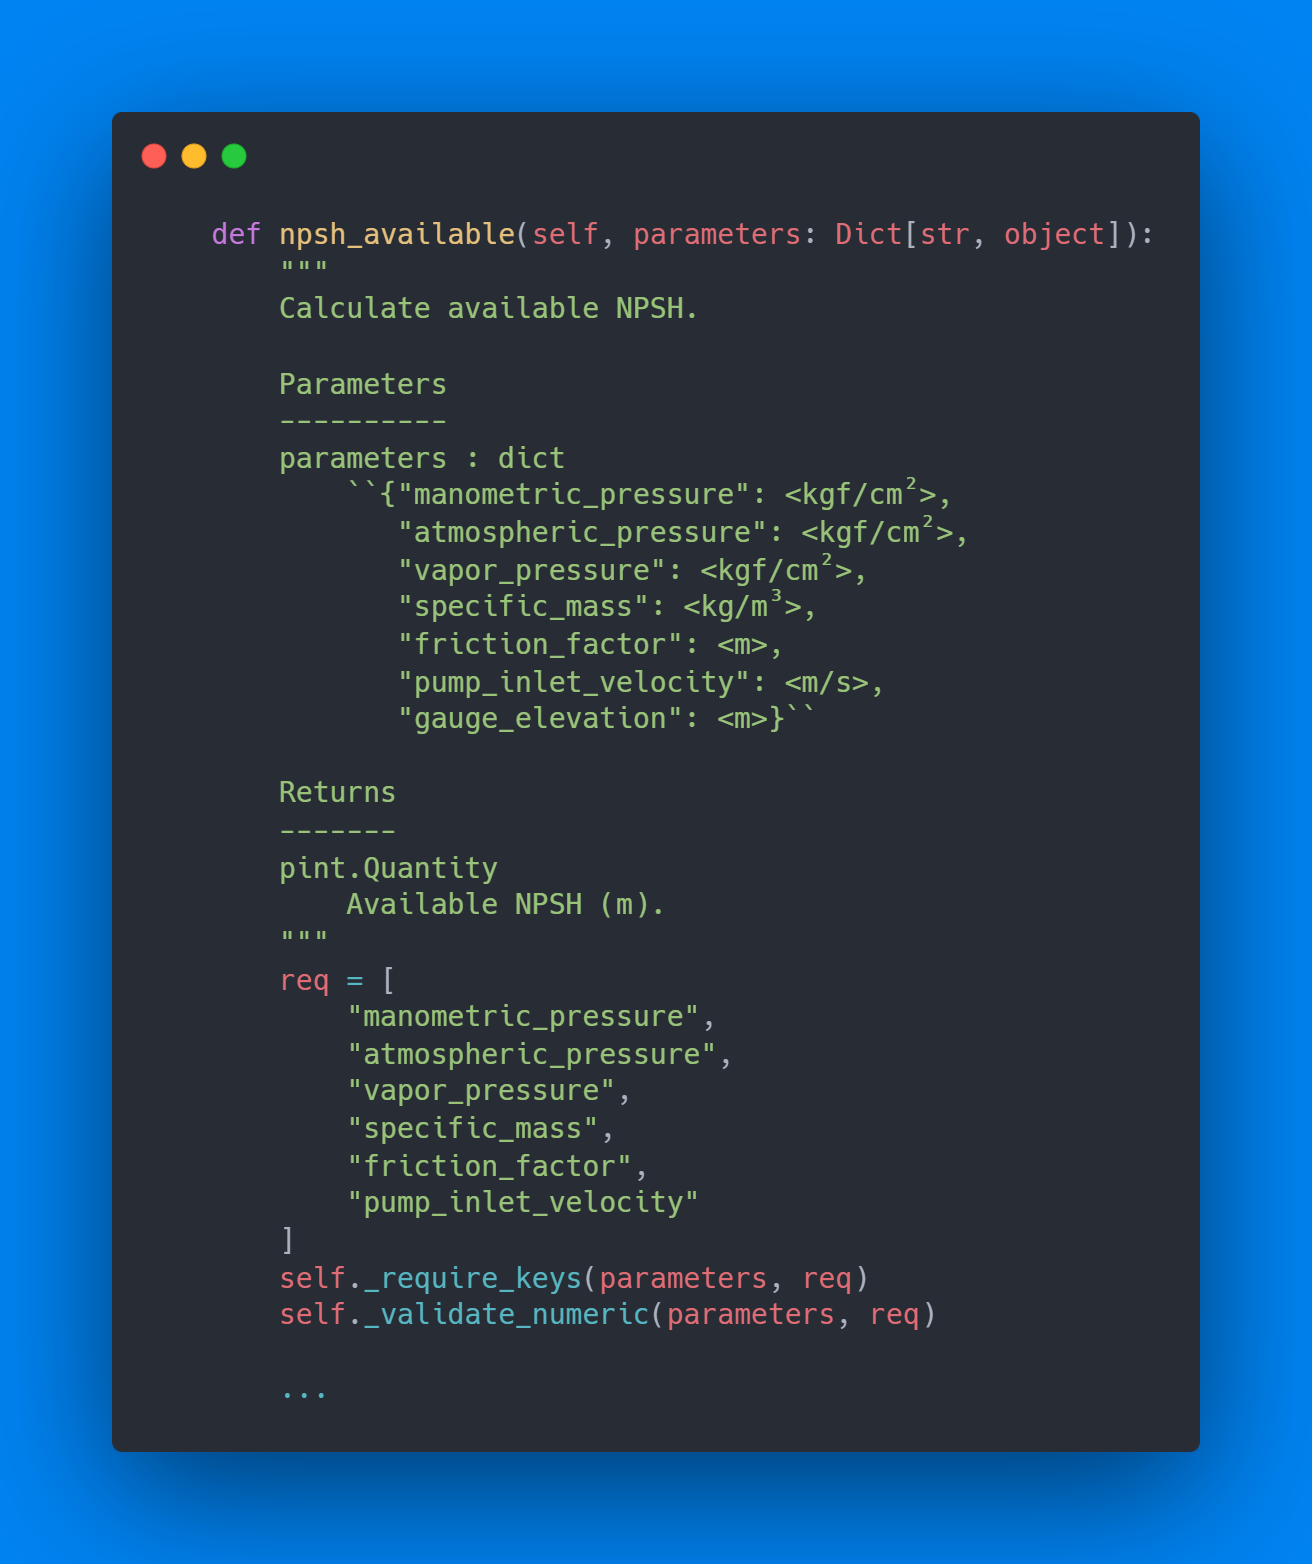
\includegraphics[width=\linewidth]{media/cap4_npsh_parte_um.png}
    \fonte{Elaboração própria (2026).}
\end{figure}

\begin{figure}[H]
    \centering
    \caption{Cálculo do \textit{NPSH} – Parte 2/2}
    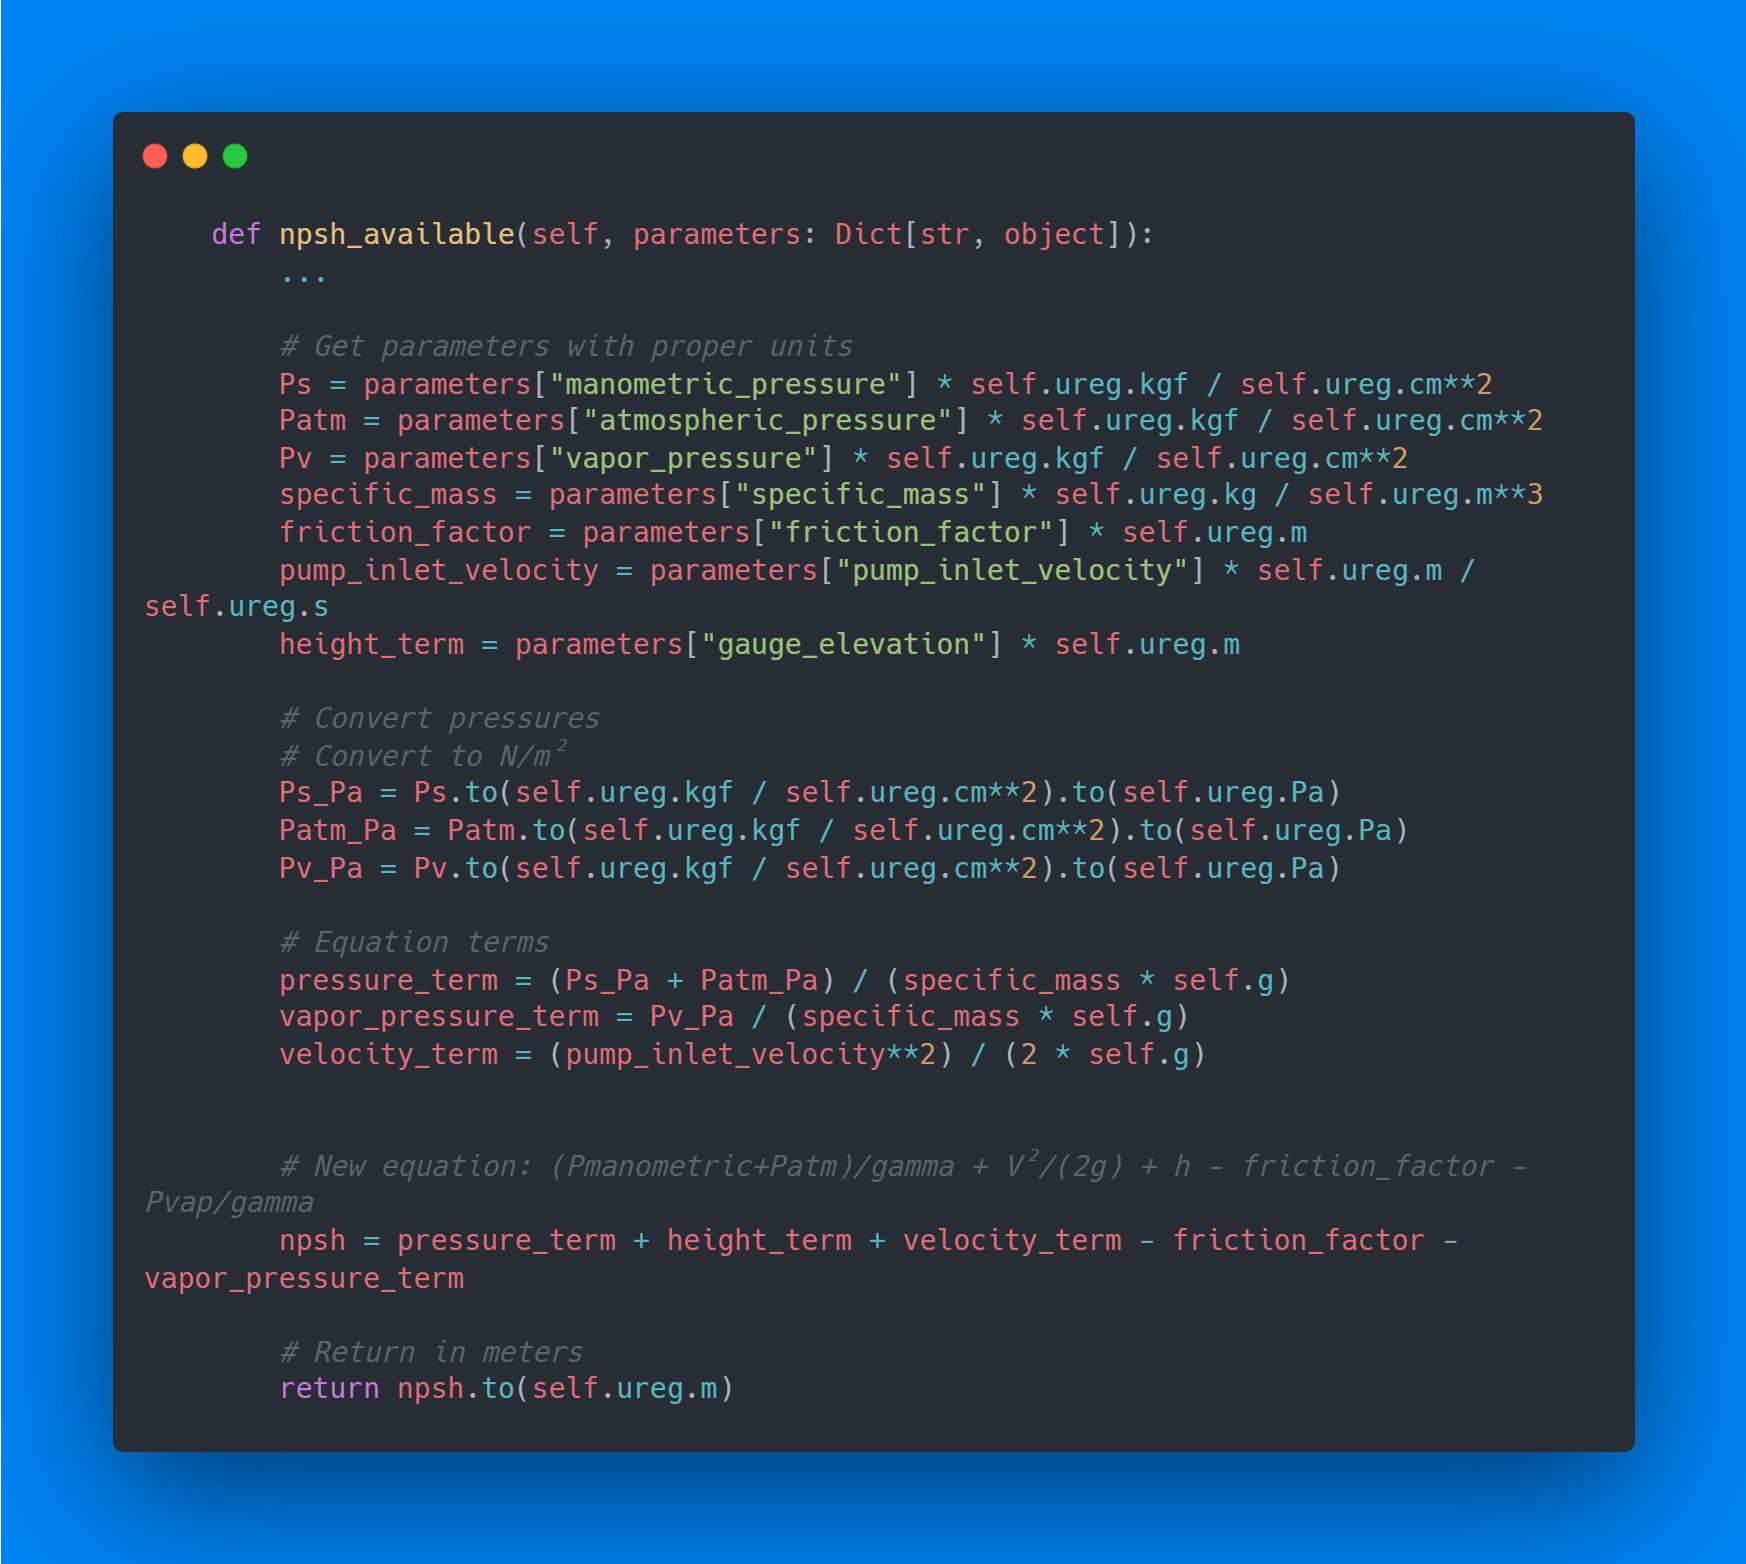
\includegraphics[width=\linewidth]{media/cap4_npsh_parte_dois.png}
    \fonte{Elaboração própria (2026).}
\end{figure}
